% Broadband Expansion and Small-Firm Productivity — 15-min conference talk.
% House theme. Compile: python3 <skill>/scripts/compile_deck.py broadband-conf-15min.tex
% All numbers carry a source tag (% Table/Fig, p.). Paper = fictional demo manuscript.
\documentclass[11pt, aspectratio=169]{beamer}
\usepackage{econ-slides-house}

% COLOR MAP (one color per concept, held for the whole talk):
%   broadband / treatment                      = cAccentC (teal; matches the paper figures)
%   communication intensity / complementarity  = cAccentA (blue)
\colorlet{cTreat}{cAccentC}
\colorlet{cMech}{cAccentA}

\title{Broadband raises small-firm productivity by 3.4 percent}
\subtitle{Evidence from a staggered municipal broadband rollout}
\author{Astrid Lindqvist \and Tomas Berg}
\date{July 2026}

\begin{document}

% ---- Title (de-counted) ----
\begin{frame}[plain]
  \titlepage
  \vfill\centering\scriptsize\textit{Demonstration manuscript; setting and data are simulated.}
\end{frame}
\addtocounter{framenumber}{-1}

% ---- 1. Motivation + question (merged for a short talk) ----
\begin{frame}[t]{Can universal broadband raise small-firm productivity?}
  \medskip
  \begin{itemize}\setlength{\itemsep}{0.7em}
    \item Small firms dominate employment but adopt technology late \graycite{(Syverson '11)}
    \item Universal broadband could compress productivity gaps at modest fiscal cost
    \vspace*{-0.5em}
    \item[$\Rightarrow$] \textbf{Does broadband causally raise small-firm productivity, and for whom?}
  \end{itemize}
  \medskip
  {\graycite{Prior evidence is aggregate or worker-level: (Czernich '13; Akerman '15; Hjort--Poulsen '19).}}
\end{frame}

% ---- 2. This paper: THE PUNCHLINE SLIDE ----
\begin{frame}[t]{This paper}
  \medskip
  We exploit the staggered municipal rollout of Nordavia's National Broadband
  Program: 284 municipalities, 9{,}400 small firms, 2008--2019.
  \medskip
  \begin{enumerate}\setlength{\itemsep}{0.9em}
    \item Broadband raises small-firm labor productivity by \KeyIdea{3.4\%} \graycite{(s.e.\ 0.2 pp)}  % Table 2, col (1), p.7
    \item Gains rise with communication intensity, as the model predicts \graycite{(0.032)}  % Table 4, col (1), p.9
    \item The program repays its build cost within six years, small firms alone  % Section 7, p.8-9
  \end{enumerate}
  \medskip
  \textbf{Implication:} among the cheapest productivity policies available to a small open economy.
\end{frame}

% ---- 3. Data ----
\begin{frame}[t]{Data}
  \medskip
  \begin{itemize}\setlength{\itemsep}{0.6em}
    \item \RunIn{Program:} Nordavian National Broadband Program, staggered 2011--2018  % Section 4.1, p.4
    \item \RunIn{Sample:} 9{,}400 firms with 3--49 employees, 2008--2019 \graycite{(112{,}800 firm-years)}  % Section 4.2, p.5
    \item \RunIn{Outcome:} log real value added per worker  % Appendix B, p.11
    \item \RunIn{Comm.\ intensity:} 2008 wage-bill share of communication jobs \graycite{(mean 0.42)}  % Table 1, p.5
  \end{itemize}
  \hypertarget{main:data}{}%
  \PlaceNav{\hyperlink{app:sumstats}{\beamergotobutton{Summary stats}}}
\end{frame}

% ---- 4. Identification: the rollout picture ----
\begin{frame}{Staggered rollout timing identifies the effect}
  \framesubtitle{Identifying assumption: arrival timing is unrelated to firms' counterfactual trends}
  \centering
  \vspace{0.3em}
  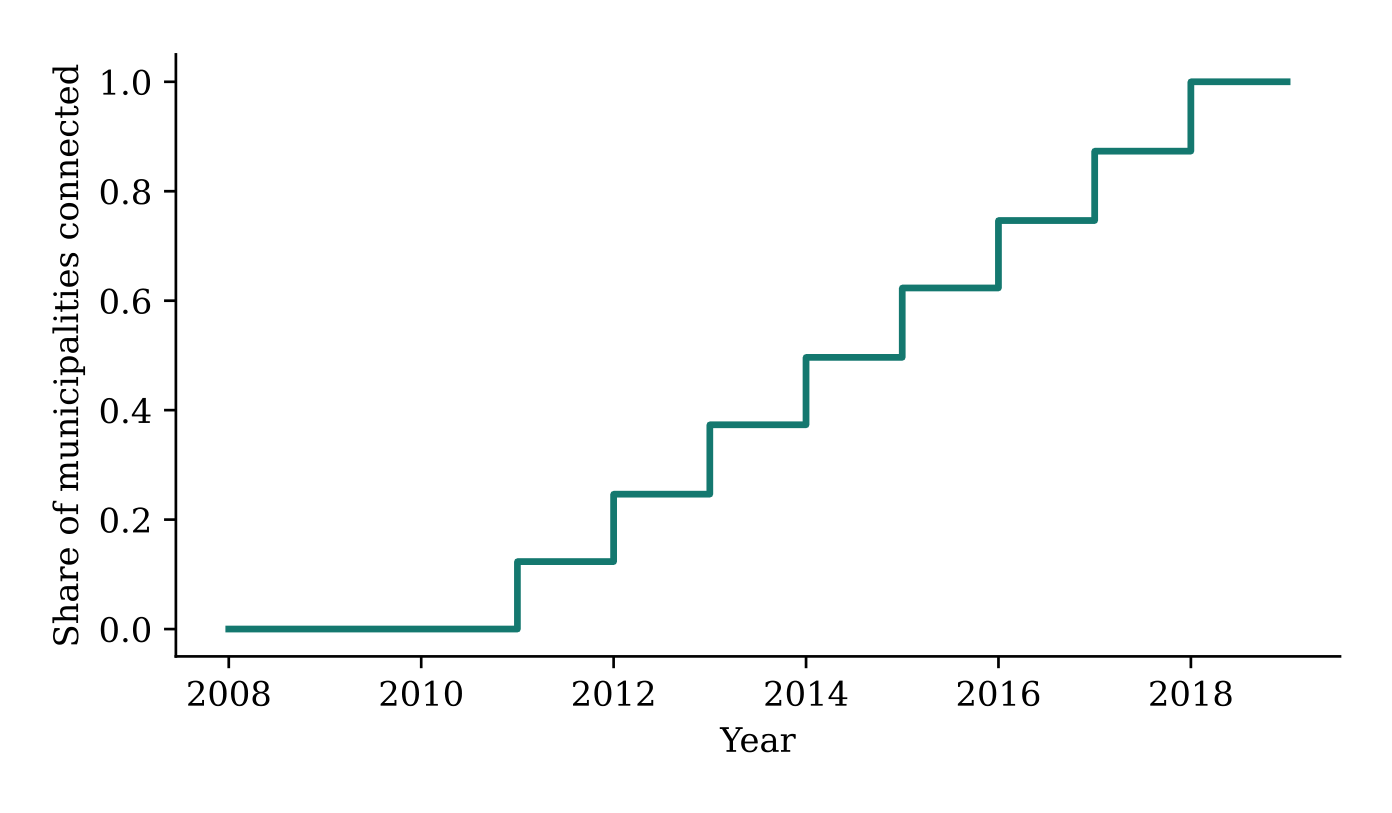
\includegraphics[width=0.70\textwidth,keepaspectratio]{figures-slides/fig1_rollout.png}  % Figure 1, p.5 (cropped)
  \Takeaway{Timing was locked by the 2010 Act, not by the scoring rule's tilt toward high-growth places.}
  \hypertarget{main:design}{}%
  \PlaceNav{\hyperlink{app:placebo}{\beamergotobutton{Placebo}}}
\end{frame}

% ---- 5. Main result: the event study (THE exhibit) ----
\begin{frame}{Effects appear only after arrival and keep building}
  \framesubtitle{Event-study coefficients vs.\ the year before arrival; 95\% CIs, firm-clustered SEs}
  \centering
  \vspace{0.2em}
  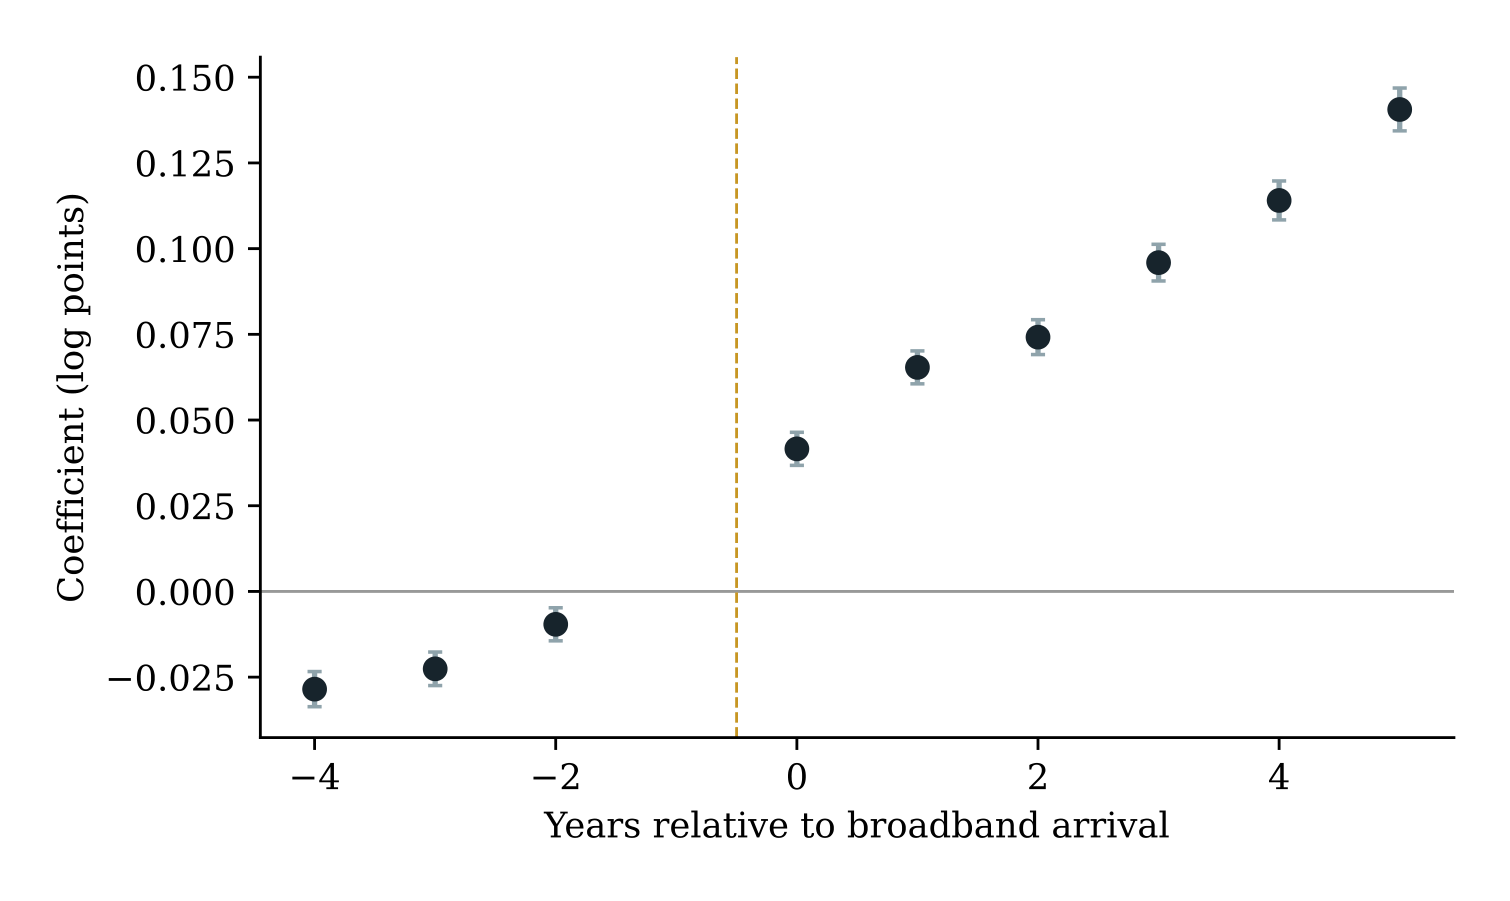
\includegraphics[width=0.64\textwidth,keepaspectratio]{figures-slides/fig2_eventstudy.png}  % Figure 2, p.7 (cropped)
  \Takeaway{No jump before arrival; the effect emerges at $t=0$ and builds. Average gain 3.4\% \graycite{(0.034, s.e.\ 0.002)}.}
  \hypertarget{main:result}{}%
  \PlaceNav{\hyperlink{app:baseline}{\beamergotobutton{Full table}}\;\hyperlink{app:robust}{\beamergotobutton{Robustness}}}
\end{frame}

% ---- 6. Mechanism: model prediction meets the interaction ----
\begin{frame}[t]{Gains concentrate where the model predicts}
  \framesubtitle{Broadband interacted with 2008 communication intensity $\theta_i$}
  \medskip
  Model prediction: firms doing more communication-intensive work gain more from
  broadband \graycite{(Prop.\ 1: $G'(\theta_i)>0$)}.
  \medskip
  \[
    y_{it}-\ell_{it} = \alpha_i + \lambda_t
      + \textcolor{cTreat}{\beta\,B_{mt}}
      + \underbrace{\textcolor{cMech}{\gamma\,(B_{mt}\times\theta_i)}}_{\text{complementarity, }\gamma>0}
      + \varepsilon_{it}
  \]
  {\small where $B_{mt}=1$ once broadband reaches firm $i$'s municipality;
  \textcolor{cTreat}{$\beta$} is the average gain, \textcolor{cMech}{$\gamma$}
  the extra gain per unit of communication intensity.\par}
  \medskip
  \begin{ResultBox}[Model confirmed]
    \textcolor{cMech}{$\hat\gamma=0.032$} (s.e.\ 0.005): a firm one SD above mean
    communication intensity gains about one-fifth more than the average firm.  % Table 4 col (1) + Section 6.3, p.8
  \end{ResultBox}
  \hypertarget{main:mech}{}%
  \PlaceNav{\hyperlink{app:model}{\beamergotobutton{Model}}\;\hyperlink{app:hetero}{\beamergotobutton{By intensity}}}
\end{frame}

% ---- 7. Conclusion: mirrors "This paper" ----
\begin{frame}[t]{Conclusion}
  \medskip
  Staggered municipal broadband, 284 municipalities and 9{,}400 small firms, 2008--2019:
  \medskip
  \begin{enumerate}\setlength{\itemsep}{0.9em}
    \item Broadband raises small-firm labor productivity by \KeyIdea{3.4\%} \graycite{(s.e.\ 0.2 pp)}  % Table 2, col (1), p.7
    \item Gains rise with communication intensity, as the model predicts \graycite{(0.032)}  % Table 4, col (1), p.9
    \item The program repays its build cost within six years, small firms alone  % Section 7, p.8-9
  \end{enumerate}
  \medskip
  \textbf{Implication:} among the cheapest productivity policies available to a small open economy.
  \hypertarget{main:concl}{}%
  \PlaceNav{\hyperlink{app:policy}{\beamergotobutton{Policy math}}}
\end{frame}
% No "Thank you / Questions?" slide.

% ================= Appendix =================
\AppendixStart

% A1 — Summary statistics
\begin{frame}{Summary statistics}
  \hypertarget{app:sumstats}{}%
  \vspace{0.6em}
  \centering
  \begin{threeparttable}
    \begin{tabular}{lrr}
      \toprule
      & Mean & SD \\ \midrule
      Log labor productivity  & 0.10  & 0.46 \\  % Table 1, p.5
      Employees               & 23.40 & 7.31 \\
      Firm age                & 21.45 & 9.56 \\
      Communication intensity & 0.42  & 0.20 \\
      ICT investment (log)    & 0.37  & 0.36 \\
      \bottomrule
    \end{tabular}
    \begin{tablenotes}\footnotesize
      \item 112{,}800 firm-year observations; 9{,}400 firms; 2008--2019. Min/max omitted.
    \end{tablenotes}
  \end{threeparttable}
  \BackButton{main:data}
\end{frame}

% A2 — Baseline estimates (full)
\begin{frame}{Baseline estimates}
  \hypertarget{app:baseline}{}%
  \framesubtitle{Dependent variable: log labor productivity; firm and year fixed effects}
  \vspace{4pt}
  \centering
  \resizebox{0.88\textwidth}{!}{%
  \begin{threeparttable}
    \begin{tabular}{lcccc}
      \toprule
      & \textcolor{cTreat}{(1) Baseline} & (2) +Controls & (3) +Region trends & (4) Muni.\ cluster \\ \midrule
      Broadband            & \textcolor{cTreat}{\textbf{0.034}} & 0.033   & 0.030   & 0.034 \\  % Table 2, p.7
                           & \textcolor{cTreat}{(0.002)}        & (0.002) & (0.002) & (0.003) \\
      ICT investment (log) &         & 0.000   &         &         \\
                           &         & (0.002) &         &         \\ \midrule
      Firm \& year FE      & Yes     & Yes     & Yes     & Yes \\
      Observations         & 112{,}800 & 112{,}800 & 112{,}800 & 112{,}800 \\
      \multicolumn{5}{l}{\textcolor{cTreat}{\footnotesize Stable across controls, region trends, and clustering.}} \\
      \bottomrule
    \end{tabular}
    \begin{tablenotes}\footnotesize
      \item SEs clustered by firm, except col.\ (4) by municipality. All coefficients significant at 1\%.
    \end{tablenotes}
  \end{threeparttable}}
  \Takeaway{The headline 3.4\% is unchanged by controls and region trends.}
  \BackButton{main:result}
\end{frame}

% A3 — Robustness
\begin{frame}{Robustness}
  \hypertarget{app:robust}{}%
  \framesubtitle{Broadband coefficient across specifications; firm and year fixed effects}
  \vspace{4pt}
  \centering
  \begin{threeparttable}
    \begin{tabular}{lccc}
      \toprule
      & (1) Region trends & (2) No controls & (3) Drop 2011--12 cohorts \\ \midrule
      Broadband & 0.030   & 0.034   & 0.037 \\  % Table 5, p.9
                & (0.002) & (0.002) & (0.002) \\
      \bottomrule
    \end{tabular}
    \begin{tablenotes}\footnotesize
      \item SEs clustered by firm. Full control set throughout. All significant at 1\%.
    \end{tablenotes}
  \end{threeparttable}
  \Takeaway{The effect stays in 0.030--0.037 across reasonable perturbations.}
  \PlaceNav{\hyperlink{app:cohort}{\beamergotobutton{By cohort}}\;\hyperlink{main:result}{\beamerreturnbutton{Back}}}
\end{frame}

% A4 — Placebo
\begin{frame}{Placebo test with permuted rollout years}
  \hypertarget{app:placebo}{}%
  \framesubtitle{Rollout years randomly permuted across municipalities; pre-treatment sample}
  \vspace{4pt}
  \centering
  \begin{threeparttable}
    \begin{tabular}{lc}
      \toprule
      & Pre-period placebo \\ \midrule
      Placebo broadband \graycite{(permuted years)} & $-0.004$ \\  % Table 3, p.8
                                                     & (0.002) \\
      \bottomrule
    \end{tabular}
    \begin{tablenotes}\footnotesize
      \item SEs clustered by firm.
    \end{tablenotes}
  \end{threeparttable}
  \Takeaway{A precisely estimated zero: no effect where none should appear.}
  \BackButton{main:design}
\end{frame}

% A5 — Cohort estimates
\begin{frame}{Effects are similar across rollout cohorts}
  \hypertarget{app:cohort}{}%
  \framesubtitle{Separate DiD estimate per cohort vs.\ municipalities connected $\geq$3 years later}
  \centering
  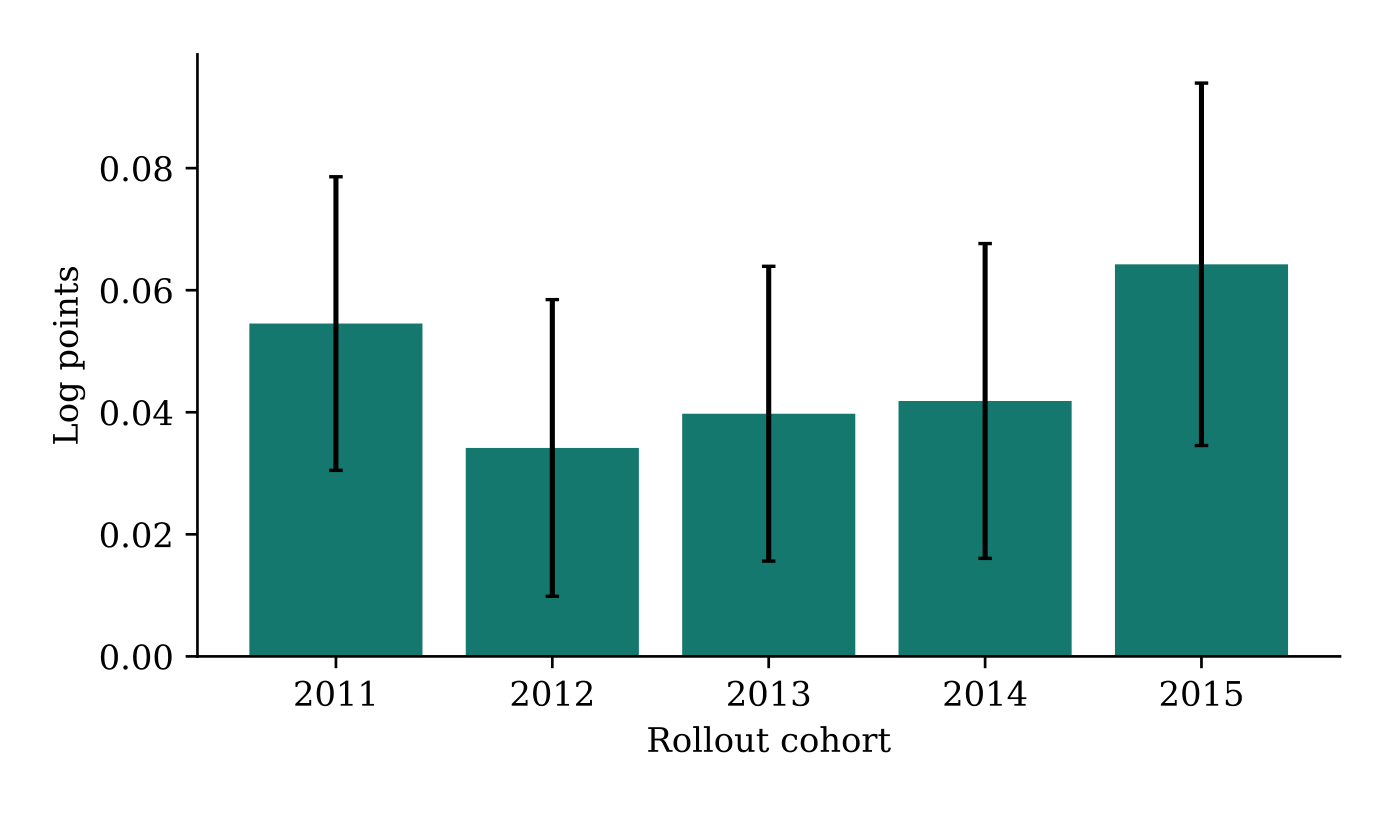
\includegraphics[width=0.62\textwidth,keepaspectratio]{figures-slides/fig3_cohort.png}  % Figure 3, p.8 (cropped)
  \Takeaway{Positive and similar across cohorts, so negative weighting is not a concern \graycite{(Goodman-Bacon '21)}.}
  \BackButton{main:result}
\end{frame}

% A6 — Heterogeneity table
\begin{frame}{Heterogeneity by communication intensity}
  \hypertarget{app:hetero}{}%
  \framesubtitle{Dependent variable: log labor productivity; firm and year fixed effects}
  \vspace{4pt}
  \centering
  \begin{threeparttable}
    \begin{tabular}{lcc}
      \toprule
      & (1) & (2) \\ \midrule
      Broadband                                             & 0.020   & 0.034 \\  % Table 4, p.9
                                                            & (0.003) & (0.002) \\
      \textcolor{cMech}{Broadband $\times$ comm.\ intensity} & \textcolor{cMech}{\textbf{0.032}} & \\
                                                            & \textcolor{cMech}{(0.005)} & \\ \midrule
      Firm \& year FE                                       & Yes     & Yes \\
      Observations                                          & 112{,}800 & 112{,}800 \\
      \bottomrule
    \end{tabular}
    \begin{tablenotes}\footnotesize
      \item Communication intensity is the 2008 wage-bill share. SEs clustered by firm. All significant at 1\%.
    \end{tablenotes}
  \end{threeparttable}
  \Takeaway{The interaction (0.032) confirms the model's complementarity prediction.}
  \BackButton{main:mech}
\end{frame}

% A7 — The model
\begin{frame}{The model}
  \hypertarget{app:model}{}%
  \framesubtitle{Task outsourcing: broadband lowers the cost of communication-intensive tasks}
  \medskip
  \begin{itemize}\setlength{\itemsep}{0.5em}
    \item Production: $Y_i = A_i\,L_i^{1-\eta}\big[(1-s_i)+\phi\,s_i\big]^{\eta}$, with $\phi>1$  % eq (1), p.2
    \item Firm outsources a share $s_i\in[0,\theta_i]$ of communication tasks at cost $\kappa p$
    \item Sourcing rule: $s_i^\ast=\theta_i$ if $\phi w \geq \kappa p$, else $0$  % eq (2), p.3
    \item Broadband lowers the communication cost $\kappa_0 \to \kappa_1 < \kappa_0$
  \end{itemize}
  \medskip
  \begin{ResultBox}[Proposition 1]
    The productivity gain is strictly increasing in communication intensity: $G'(\theta_i)>0$.  % p.3
  \end{ResultBox}
  \BackButton{main:mech}
\end{frame}

% A8 — Policy arithmetic
\begin{frame}[t]{Policy arithmetic}
  \hypertarget{app:policy}{}%
  \medskip
  \begin{itemize}\setlength{\itemsep}{0.7em}
    \item Aggregate small-firm gain: about 410 million euros per year \graycite{(valued at 2019 value added)}  % Section 7, p.8
    \item Program construction cost: 2.3 billion euros \graycite{(RDDF cumulative)}  % Section 7, p.9
    \vspace*{-0.5em}
    \item[$\Rightarrow$] Payback within six years through the small-firm channel alone
  \end{itemize}
  \BackButton{main:concl}
\end{frame}

% A9 — Related literature (deploy only if asked)
\begin{frame}{Related literature}
  \framesubtitle{Deployed only if asked}
  \medskip
  \begin{itemize}\setlength{\itemsep}{0.6em}
    \item Czernich et al.\ (2013): broadband and aggregate growth; not the firm margin
    \item Akerman et al.\ (2015): broadband is skill-complementary; worker-level, larger firms
    \item Hjort and Poulsen (2019): fast internet and employment in Africa
  \end{itemize}
  \medskip
  This paper: the small-firm segment in an advanced economy, tied to an explicit task-outsourcing model.
\end{frame}

\end{document}
